% -----------------------------------------------
\section{Methodology}
% -----------------------------------------------

\begin{frame}{System Overview}
  \begin{figure}
    \centering
    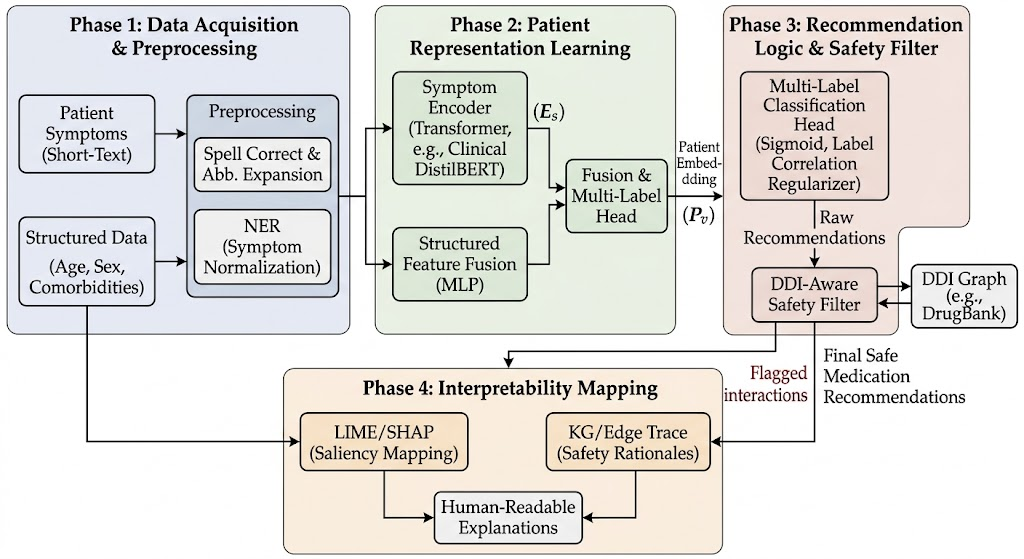
\includegraphics[trim={0.1in 0.1in 0.1in 1in}, clip, width=\linewidth]{figures/architecture.png}
    \caption{Four-phase medication recommendation pipeline.}
  \end{figure}
  \note{Walk through the figure -- four phases: preprocessing, representation learning, recommendation + safety, interpretability.}
\end{frame}

\begin{frame}{Preprocessing \& Patient Representation}
  \textbf{Input:} Free-text symptoms + age, sex, comorbidities
  \pause
  \begin{itemize}
    \item Spell correction, abbreviation expansion (e.g., SOB $\to$ Shortness of Breath)
    \item NER $\to$ SNOMED-CT / ICD-10 entity mapping
    \pause
    \item \textbf{Symptom embedding $E_s$:} Clinical DistilBERT
    \item \textbf{Structured embedding $E_d$:} MLP over demographics \& comorbidities
    \item \textbf{Patient state:} $P_v = \text{Concatenate}(E_s,\, E_d)$
  \end{itemize}
  \note{Stress that DistilBERT is lightweight by design -- important for outpatient/low-latency settings.}
\end{frame}

\begin{frame}{Recommendation \& Safety Filtering}
  \begin{itemize}
    \item Multi-label sigmoid head over $P_v$ $\to$ per-drug-class probabilities
    \item Label-correlation regularizer for co-prescription dependencies
    \pause
    \item Top-$k$ candidates passed to \textbf{DDI-aware safety filter} (DrugBank graph)
    \item Unsafe combinations $\to$ penalized in ranking or clinician alert
  \end{itemize}
  \note{The safety filter is the key differentiator from vanilla multi-label classifiers. Mention the override alert for clinical trust.}
\end{frame}

\begin{frame}{Interpretability}
  \begin{itemize}
    \item \textbf{SHAP saliency:} token-level attribution over symptom text
    \pause
    \item \textbf{Safety rationales:} knowledge-graph trace for flagged DDIs\\
    {\small e.g., \textit{``Drug A and Drug B both inhibit CYP3A4''}}
  \end{itemize}
  \note{Two layers of explainability -- one for the recommendation, one for the safety alert. Both aimed at clinician trust.}
\end{frame}

\begin{frame}{Algorithm}
  \begin{algorithm}[H]
  \caption{DL Medication Recommendation}
  \begin{algorithmic}[1]
    \REQUIRE $S$ (symptom text), $D$ (structured data), $G$ (DDI graph)
    \ENSURE $M_{safe}$, explanation report $E$
    \STATE Normalize $S$: spell correction + NER $\to$ ontology mapping
    \STATE $E_s \leftarrow$ ClinicalDistilBERT$(S)$;\quad $E_d \leftarrow$ MLP$(D)$
    \STATE $P_v \leftarrow \text{Concatenate}(E_s, E_d)$
    \STATE Sigmoid classifier $\to$ top-$k$ candidates
    \STATE DDI safety filter over $G$ $\to$ $M_{safe}$
    \STATE SHAP attribution $\to$ $E$
    \RETURN $M_{safe}$, $E$
  \end{algorithmic}
  \end{algorithm}
  \note{Condensed from the full algorithm -- hit the key steps. Good slide to have open during Q\&A.}
\end{frame}

% -----------------------------------------------
\section{Evaluation Plan}
% -----------------------------------------------

\begin{frame}{Evaluation Plan}
  \begin{itemize}
    \item \textbf{Data:} Synthea synthetic outpatient records + DrugBank / TWOSIDES
    \pause
    \item \textbf{Metrics:}
    \begin{itemize}
      \item Recommendation: Jaccard index, mean average precision
      \item Safety: DDI occurrence rate
      \item Interpretability: clinician-rated explanation utility
    \end{itemize}
    \pause
    \item \textbf{Ablations:} encoder variants, safety-layer removal, explanation fidelity
  \end{itemize}
  \note{We haven't run experiments yet -- frame this as the planned evaluation. Be ready for questions on dataset size and clinician study design.}
\end{frame}

% -----------------------------------------------
\section{Experimental Setup}
% -----------------------------------------------

\begin{frame}{Dataset}
  \begin{itemize}
    \item Synthetic outpatient encounters built from multiple public sources:
      symptom--disease, drug--disease, DDI mappings + Synthea demographics
    \pause
    \item \textbf{50,000 samples} with multi-label medication outputs
    \item Structured attributes: age (1--90), sex, comorbidity flags (diabetes, hypertension, asthma)
    \pause
    \item Text augmentation: synonym replacement, template sentences
    \item DDI filtering + clinical heuristics (e.g., no ibuprofen for hypertensive patients)
  \end{itemize}
  \note{Stress that the dataset is synthetic but clinically grounded. The DDI filtering means ground-truth labels are already safe -- important context for interpreting the DDI rate metric.}
\end{frame}

\begin{frame}{Models Compared}
  \begin{table}
    \centering
    \begin{tabular}{ll}
      \hline
      \textbf{Model} & \textbf{Key Design Choice} \\
      \hline
      MLP            & Flattened token embeddings + structured features \\
      TextCNN        & 1D filters over embeddings, local $n$-gram features \\
      BiLSTM         & Bidirectional sequence encoding \\
      SelfAttention  & Single-head attention + mean pooling \\
      \textbf{FusionNet} & \textbf{LSTM (text) + MLP (structured), dual-branch} \\
      \hline
    \end{tabular}
  \end{table}
  \pause
  \begin{itemize}
    \item Shared: 64-dim embeddings, max sequence length 20, BCE loss
    \item Adam, lr $= 10^{-3}$, 5 epochs, batch size 32, 80/20 split
  \end{itemize}
  \note{The table cleanly shows the progression in complexity. FusionNet is the only model with an explicit dual-branch design -- that's the hypothesis being tested.}
\end{frame}

\begin{frame}{Evaluation Metrics}
  \begin{itemize}
    \item \textbf{Multi-label quality:} Jaccard index, micro-F1, subset accuracy, Hamming loss
    \item \textbf{Ranking} ($k=5$): Precision@$K$, Recall@$K$, F1@$K$, PR-AUC
    \item \textbf{Discrimination:} ROC-AUC (micro)
    \pause
    \item \textbf{Safety:} DDI rate -- fraction of top-$k$ pairs with known adverse interactions
  \end{itemize}
  \note{Highlight the DDI rate -- it's the only metric that directly measures safety, and it's what distinguishes this work from standard multi-label classification.}
\end{frame}
